\documentclass{article}
\title{\Huge Numerical Methods}
\Large{\author{$\mathcal{WAFFLE'S\ \ CRAZY\ \ PEANUT}$}}
\date{(Last updated: 26/3/14)}
\usepackage{enumerate}
\usepackage{tikz}
\usepackage[utf8]{inputenc}
\usepackage[T1]{fontenc}
\usepackage[margin=1in]{geometry}
\usetikzlibrary{shadows,trees}
\usepackage{tikz-qtree,tikz-qtree-compat}
\usetikzlibrary{trees}
\usepackage{amsmath}
\newcommand{\para}[1]{\paragraph{#1}\mbox{}\\}
\usetikzlibrary{decorations.pathreplacing}
\pagenumbering{gobble}
\begin{document}
\maketitle
\textbf{\section{\huge Solution of Equations:}}
\
{\Large 
\subsection{\LARGE Fixed-point Iteration:}
Iterate within the limits of roots.
\paragraph{\Large Procedure:}
\begin{enumerate}[(i)]
\item Identify whether the given {\LARGE $f(x)$} is linear algebraic, non-linear algebraic, or transcendental equation.
\item Start finding $f(0),\ f(1),\ ...$ until there's a change of sign in the value, which corresponds to the limit $(a,b)$ within which the root lies.
\item Write the function in the form {\LARGE $\ x=\phi(x)$}
\item Check the condition {\LARGE $|\phi'(a)|$} $<1$ and {\LARGE $|\phi'(b)|$}$<1$
\item Now, find $x_0,\ x_1=\phi(x_0),\ x_2=\phi(x_1),\ ...$ for values lying in the limit $(a,b)$ and stop when the repetition of rounded values occurs.
\end{enumerate}
\newpage
\paragraph{\Large Note: } For infinite series, as there's no specific interval, find the roots directly by taking {\LARGE $x=f(x)$}, neglecting higher powers, and iterating using step (v).

\paragraph{\Large Keep in mind}Root-finding will be easier if iterations begin with the value nearer to $a$ or $b$, based on whether $|f(a)|$ or $|f(b)|$ is closer to zero.
\\
\\
If $f(a)$ is closer to zero, then the root is closer to $a$, and vice versa.
\subsection{\LARGE Newton-Raphson Method:}
{\LARGE $$x_{n+1}=x_n-\frac{f(x_n)}{f'(x_n)}$$}
\textbf{Procedure:}
\begin{enumerate}[(i)]
\item Identify whether the given {\LARGE $f(x)$} is linear algebraic, non-linear algebraic, or transcendental equation.
\item Start finding $f(0),\ f(1),\ ...$ until there's a change of sign in the value, which corresponds to the limit $(a,b)$ within which the root lies.
\item Now, find $x_0$, $x_1$, $x_2$... using the iterative formula, and proceed until repetition occurs.
\end{enumerate}
\paragraph{\Large Some formulas (can be derived):}
\begin{itemize}
\item If {\LARGE $\ x=$} {\huge $\frac{1}N$},
{\LARGE $$x_{n+1}=x_n(2-Nx_n)$$}
\item If {\LARGE $\ x=\sqrt{N},$}
{\LARGE $$x_{n+1}=\frac{1}2\bigg(x_n+\frac{N}{x_n}\bigg)$$}
\item If {\LARGE $\ x=$} {\huge $\frac{1}{\sqrt{N}}$} ,
{\LARGE $$x_{n+1}=\frac{1}2\bigg(x_n+\frac{1}{Nx_n}\bigg)$$}
\item If {\LARGE $\ x=N^{1/k}$} ,
{\LARGE $$x_{n+1}=\frac{1}k\bigg((k-1)x_n+\frac{N}{x_n^{k-1}}\bigg)$$}
\end{itemize}
$\ $
\subsection{\LARGE Solution of linear system of equations:}
$\ $
\tikzset{font=\Large,
edge from parent fork down,
level distance=2cm,
every node/.style=
    {top color=white,
    rectangle,rounded corners,
    minimum height=1cm,
    draw=black!50,
    very thick,
    drop shadow,
    align=center,
    text depth = 1pt
    },
edge from parent/.style=
    {draw=black!50,
    thick}}
\begin{center}
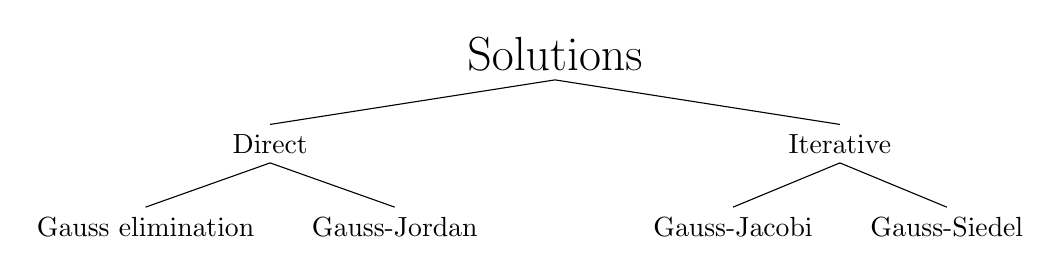
\begin{tikzpicture}[level 1/.style={sibling distance=2cm},level 2/.style={sibling distance=0.5cm}]
\Tree [.{\LARGE Solutions}
        [.{Direct}
            [.{Gauss elimination} ]
            [.{Gauss-Jordan} ] ] 
        [.Iterative
            [.{Gauss-Jacobi} ]
            [.{Gauss-Siedel} ] ] 
]
\end{tikzpicture}
\end{center}
}\end{document}